\documentclass[12pt,a4paper]{article}
\title{MATH1110 Lec 009 Week 6-W}
\author{Benjamin Thompson}
\date{September 29, 2021}

\usepackage[left=2cm,right=2cm]{geometry}

\usepackage{tikz, tikz-3dplot}
\usetikzlibrary{arrows.meta,decorations.markings}
\usepackage{etoolbox}

\usepackage{pgfplots}

\pgfplotsset{every axis/.append style={
axis x line=middle,    % put the x axis in the middle
axis y line=middle,    % put the y axis in the middle
axis line style={-{Stealth[length=3mm]},color=black}, % arrows on the axis
minor tick num=1
}}

\usepackage{amsmath}
\usepackage{graphicx}

\usepackage{fancyhdr}
\pagestyle{fancy}

\newcommand{\rar}{\rightarrow}

\fancyhf{}
\lhead{MATH1110 Sec 009}
\chead{Week 6-W}
\rhead{September 29, 2021}
\cfoot{}

\begin{document}
\section*{Practice Quiz and Solutions}
\subsection*{Questions}
\begin{enumerate}
    \item Evaluate
    \[
        \lim_{x \rightarrow 0} \frac{(1-\cos x)(1+\cos x)}{x}
    \]
    if it exists. If it does not, explain why.
    
    \item Find all values $a$ for which the tangent line to the curve $y = x(x+1)^2$ at $x=a$ is horizontal.
    
    \item Let $f(x) = \sin(x)/x$ when $x \ne 0$, and $f(0) = 1$. Is $f$ differentiable at $x=0$?
   % \item Does $(pq)' = p'q'$ for all polynomials $p(x),q(x)$? If not, give a pair of polynomials $(a(x),b(x))$ for which $(ab)' \ne a'b'$. 
    
    \item Does $(pq)' = p'q'$ for any polynomials $p(x),q(x)?$ If so, give a pair of polynomials $(a(x),b(x))$ for which $(ab)' = a'b'$.
    
    \item A polynomial $p(x)$, as well as its derivative $p'(x)$ and second derivative $p''(x)$ are plotted below. Match $p,p',p''$ with $A,B,C$.
\[
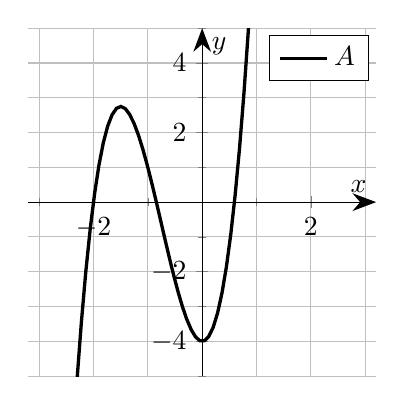
\begin{tikzpicture}
\begin{axis}[xlabel={$x$},ylabel={$y$},width=6cm, height=6cm, xmin=-3.2,xmax=3.2, ymin=-5,ymax=5, grid=both]
\addplot [very thick, domain=-4:4,samples=100]{4*x^3 + 9*x^2 - 4};
\addlegendentry{$A$}
\end{axis}
\end{tikzpicture}
\quad
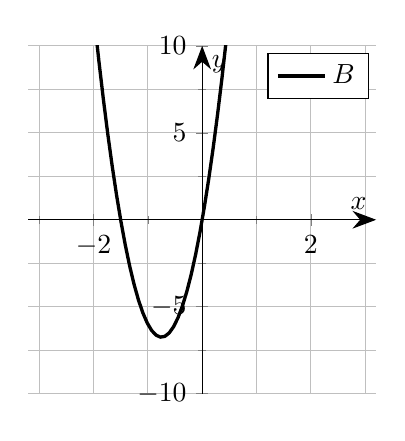
\begin{tikzpicture}
\begin{axis}[xlabel={$x$},ylabel={$y$},width=6cm, height=6cm, xmin=-3.2,xmax=3.2, ymin=-10,ymax=10, grid=both]
\addplot [very thick, domain=-4:4,samples=100]{6*x*(2*x+3)};
\addlegendentry{$B$}
\end{axis}
\end{tikzpicture}
\quad
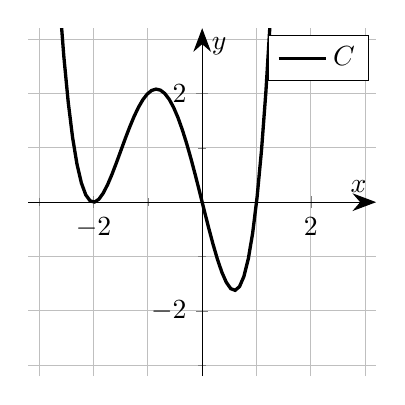
\begin{tikzpicture}
\begin{axis}[xlabel={$x$},ylabel={$y$},width=6cm, height=6cm, xmin=-3.2,xmax=3.2, ymin=-3.2,ymax=3.2, grid=both]
\addplot [very thick, domain=-4:4,samples=100]{x*(x+2)^2*(x-1)};
\addlegendentry{$C$}
\end{axis}
\end{tikzpicture}
\]
\end{enumerate}

\subsection*{Solutions}
\begin{enumerate}
	\item Note that
\[
	(1 - \cos x)(1 + \cos x) = 1 - \cos^2 x.
\]
Rearranging the identity $\sin^2 x + \cos^2 x = 1$ gives $\sin^2 x = 1 - \cos^2 x$. Therefore
\[
	\lim_{x \rar 0}\frac{(1 - \cos x)(1 + \cos x)}{x} = \frac{\sin^2x}{x} = \lim_{x \rar 0} \left( \frac{\sin x}{x} \cdot \sin x \right).
\]
Now
\[
	\lim_{x \rar 0}\frac{\sin x}{x} = 1, \qquad \lim_{x \rar 0}\sin x = \sin 0 = 0,
\]
so since both of these exist we can apply the limit product law to conclude
\[
	\lim_{x \rar 0}\left( \frac{\sin x}{x} \cdot \sin x \right) = \lim_{x \rar 0}\frac{\sin x}{x} \cdot \lim_{x \rar 0} \sin x = 1 \cdot 0 = 0.
\]
	\item The curve $y = x(x+1)^2$ will have a horizontal tangent when the derivative of $f(x) = x(x+1)^2$ is zero. We could calculate $f'$ using the product rule, but the calculation is probably easier if we expand it first.
\[
	x(x+1)^2 = x(x^2 + 2x + 1) = x^3 + 2x^2 + x.
\]
Hence
\[
	f'(x) = (x^3 + 2x^2 + x)' = 3x^2 + 4x + 1 = (3x + 1)(x+1).
\]
Hence $f'(x) = 0$ when $3x + 1 = 0$ or $x + 1 = 0$, i.e when $x = -1/3, -1$, so the possible values of $a$ are $-1/3$ and $-1$.
	\item A limit used in Q1 implies that this function is continuous at $x = 0$, so it is at least plausible that the function is differentiable at $x = 0$. (If a function is not continuous at a point, it is not differentiable at that point.) We can use the limit definition to see if the function is differentiable at $x = 0$:
\begin{equation*}
\begin{split}
	\lim_{h \rar 0}\frac{f(0 + h) - f(0)}{h} &= \lim_{h \rar 0}\frac{\frac{\sin(h)}{h} - 1}{h}  \\
		&= \lim_{h \rar 0}\left( \frac{\sin(h) - h}{h^2} \right).
\end{split}
\end{equation*}
If you graph this function it is clear that the limit exists and should be 0,\ldots but there is no simple way of showing this algebraically. The easiest way forwards is by using L'H\^opital's rule, a theorem we will cover later in the course. (NOTE: this rule \emph{will not} be covered on Prelim 1. It will also not appear on the Friday quiz!\ldots I underestimated the tools needed for this limit.)

We'll revisit this later in the course, but briefly, L'H\^opital's rule means the calculations

\[
	\frac{(\sin h - h)'}{(h^2)'} = \frac{\cos h - 1}{2h},\qquad \frac{(\cos h - 1)'}{(2h)'} = -\frac{1}{2}\sin h, \qquad \lim_{h \rar 0}\frac{1}{2}\sin h = 0 
\] 
imply that the limit exists and is 0. Hence $f$ is differentiable at 0.
	\item The statement is not true in general (differentiation is not multiplicative), but the statement is true for our favorite example the constant function! Let $a(x) = b(x) =  0$.  Then $(ab)' = (0)' = 0 = 0 \cdot 0 = a'b'$.
	\item Note that on the interval $[-3,3]$, $A$, $B$ and $C$ have 2, 1, 3 points with horizontal tangent lines respectively. Therefore $A',B',C'$ have 2, 1, 3 distinct zeros in the interval $[-3,3]$ respectively. Counting the number of times the graphs cross the horizontal axis, $A,B,C$ have $3,2,3$ distinct zeros in the interval $[-3,3]$ respectively. So if neither $A$ nor $C$ have the same number of distinct zeros as $B'$ in $[-3,3]$, then $B' \ne A$ and $B' \ne C$, so we must have $B = p''(x)$.

Then either $A' = C$ or $A = C'$. Note that $A'$ has two distinct zeros in $[-3,3]$, while $C$ has 3 distinct zeros in $[-3,3]$. This means $A' \ne C$, so we conclude $A = C'$. Therefore $(A,B,C) = (p',p'',p)$.


\end{enumerate}

\end{document}
